\documentclass[]{book}
\usepackage{lmodern}
\usepackage{amssymb,amsmath}
\usepackage{ifxetex,ifluatex}
\usepackage{fixltx2e} % provides \textsubscript
\ifnum 0\ifxetex 1\fi\ifluatex 1\fi=0 % if pdftex
  \usepackage[T1]{fontenc}
  \usepackage[utf8]{inputenc}
\else % if luatex or xelatex
  \ifxetex
    \usepackage{mathspec}
  \else
    \usepackage{fontspec}
  \fi
  \defaultfontfeatures{Ligatures=TeX,Scale=MatchLowercase}
\fi
% use upquote if available, for straight quotes in verbatim environments
\IfFileExists{upquote.sty}{\usepackage{upquote}}{}
% use microtype if available
\IfFileExists{microtype.sty}{%
\usepackage{microtype}
\UseMicrotypeSet[protrusion]{basicmath} % disable protrusion for tt fonts
}{}
\usepackage{hyperref}
\hypersetup{unicode=true,
            pdftitle={R for the Excel User},
            pdfauthor={Julie Lowndes \& Allison Horst},
            pdfborder={0 0 0},
            breaklinks=true}
\urlstyle{same}  % don't use monospace font for urls
\usepackage{natbib}
\bibliographystyle{apalike}
\usepackage{color}
\usepackage{fancyvrb}
\newcommand{\VerbBar}{|}
\newcommand{\VERB}{\Verb[commandchars=\\\{\}]}
\DefineVerbatimEnvironment{Highlighting}{Verbatim}{commandchars=\\\{\}}
% Add ',fontsize=\small' for more characters per line
\usepackage{framed}
\definecolor{shadecolor}{RGB}{248,248,248}
\newenvironment{Shaded}{\begin{snugshade}}{\end{snugshade}}
\newcommand{\AlertTok}[1]{\textcolor[rgb]{0.94,0.16,0.16}{#1}}
\newcommand{\AnnotationTok}[1]{\textcolor[rgb]{0.56,0.35,0.01}{\textbf{\textit{#1}}}}
\newcommand{\AttributeTok}[1]{\textcolor[rgb]{0.77,0.63,0.00}{#1}}
\newcommand{\BaseNTok}[1]{\textcolor[rgb]{0.00,0.00,0.81}{#1}}
\newcommand{\BuiltInTok}[1]{#1}
\newcommand{\CharTok}[1]{\textcolor[rgb]{0.31,0.60,0.02}{#1}}
\newcommand{\CommentTok}[1]{\textcolor[rgb]{0.56,0.35,0.01}{\textit{#1}}}
\newcommand{\CommentVarTok}[1]{\textcolor[rgb]{0.56,0.35,0.01}{\textbf{\textit{#1}}}}
\newcommand{\ConstantTok}[1]{\textcolor[rgb]{0.00,0.00,0.00}{#1}}
\newcommand{\ControlFlowTok}[1]{\textcolor[rgb]{0.13,0.29,0.53}{\textbf{#1}}}
\newcommand{\DataTypeTok}[1]{\textcolor[rgb]{0.13,0.29,0.53}{#1}}
\newcommand{\DecValTok}[1]{\textcolor[rgb]{0.00,0.00,0.81}{#1}}
\newcommand{\DocumentationTok}[1]{\textcolor[rgb]{0.56,0.35,0.01}{\textbf{\textit{#1}}}}
\newcommand{\ErrorTok}[1]{\textcolor[rgb]{0.64,0.00,0.00}{\textbf{#1}}}
\newcommand{\ExtensionTok}[1]{#1}
\newcommand{\FloatTok}[1]{\textcolor[rgb]{0.00,0.00,0.81}{#1}}
\newcommand{\FunctionTok}[1]{\textcolor[rgb]{0.00,0.00,0.00}{#1}}
\newcommand{\ImportTok}[1]{#1}
\newcommand{\InformationTok}[1]{\textcolor[rgb]{0.56,0.35,0.01}{\textbf{\textit{#1}}}}
\newcommand{\KeywordTok}[1]{\textcolor[rgb]{0.13,0.29,0.53}{\textbf{#1}}}
\newcommand{\NormalTok}[1]{#1}
\newcommand{\OperatorTok}[1]{\textcolor[rgb]{0.81,0.36,0.00}{\textbf{#1}}}
\newcommand{\OtherTok}[1]{\textcolor[rgb]{0.56,0.35,0.01}{#1}}
\newcommand{\PreprocessorTok}[1]{\textcolor[rgb]{0.56,0.35,0.01}{\textit{#1}}}
\newcommand{\RegionMarkerTok}[1]{#1}
\newcommand{\SpecialCharTok}[1]{\textcolor[rgb]{0.00,0.00,0.00}{#1}}
\newcommand{\SpecialStringTok}[1]{\textcolor[rgb]{0.31,0.60,0.02}{#1}}
\newcommand{\StringTok}[1]{\textcolor[rgb]{0.31,0.60,0.02}{#1}}
\newcommand{\VariableTok}[1]{\textcolor[rgb]{0.00,0.00,0.00}{#1}}
\newcommand{\VerbatimStringTok}[1]{\textcolor[rgb]{0.31,0.60,0.02}{#1}}
\newcommand{\WarningTok}[1]{\textcolor[rgb]{0.56,0.35,0.01}{\textbf{\textit{#1}}}}
\usepackage{longtable,booktabs}
\usepackage{graphicx,grffile}
\makeatletter
\def\maxwidth{\ifdim\Gin@nat@width>\linewidth\linewidth\else\Gin@nat@width\fi}
\def\maxheight{\ifdim\Gin@nat@height>\textheight\textheight\else\Gin@nat@height\fi}
\makeatother
% Scale images if necessary, so that they will not overflow the page
% margins by default, and it is still possible to overwrite the defaults
% using explicit options in \includegraphics[width, height, ...]{}
\setkeys{Gin}{width=\maxwidth,height=\maxheight,keepaspectratio}
\IfFileExists{parskip.sty}{%
\usepackage{parskip}
}{% else
\setlength{\parindent}{0pt}
\setlength{\parskip}{6pt plus 2pt minus 1pt}
}
\setlength{\emergencystretch}{3em}  % prevent overfull lines
\providecommand{\tightlist}{%
  \setlength{\itemsep}{0pt}\setlength{\parskip}{0pt}}
\setcounter{secnumdepth}{5}
% Redefines (sub)paragraphs to behave more like sections
\ifx\paragraph\undefined\else
\let\oldparagraph\paragraph
\renewcommand{\paragraph}[1]{\oldparagraph{#1}\mbox{}}
\fi
\ifx\subparagraph\undefined\else
\let\oldsubparagraph\subparagraph
\renewcommand{\subparagraph}[1]{\oldsubparagraph{#1}\mbox{}}
\fi

%%% Use protect on footnotes to avoid problems with footnotes in titles
\let\rmarkdownfootnote\footnote%
\def\footnote{\protect\rmarkdownfootnote}

%%% Change title format to be more compact
\usepackage{titling}

% Create subtitle command for use in maketitle
\providecommand{\subtitle}[1]{
  \posttitle{
    \begin{center}\large#1\end{center}
    }
}

\setlength{\droptitle}{-2em}

  \title{R for the Excel User}
    \pretitle{\vspace{\droptitle}\centering\huge}
  \posttitle{\par}
    \author{Julie Lowndes \& Allison Horst}
    \preauthor{\centering\large\emph}
  \postauthor{\par}
      \predate{\centering\large\emph}
  \postdate{\par}
    \date{2019-09-26}

\usepackage{booktabs}

\begin{document}
\maketitle

{
\setcounter{tocdepth}{1}
\tableofcontents
}
\hypertarget{welcome}{%
\chapter{Welcome}\label{welcome}}

Excel is a widely used and powerful tool for working with data. As automation, reproducibility, collaboration, and frequent reporting become increasingly expected in data analysis, a good option for Excel users is to extend their workflows with R. Integrating R into data analysis with Excel can bridge the technical gap between collaborators using either software. R enables use of existing tools built for specific tasks and overcomes some limitations that arise when working with large datasets or repeated analyses. This course is for Excel users who want to add or integrate R and RStudio into their existing data analysis toolkit. Participants will get hands-on experience working with data across R, Excel, and Google Sheets, focusing on: data import and export, basic wrangling, visualization, and reporting with RMarkdown. Throughout, we will emphasize conventions and best practices for working reproducibly and collaboratively with data, including naming conventions, documentation, organization, all while ``keeping the raw data raw''. Whether you are working in Excel and want to get started in R, already working in R and want tools for working more seamlessly with collaborators who use Excel, or whether you are new to data analysis entirely, this is the course for you!

If you answer yes to these questions, this course is for you!

\begin{itemize}
\tightlist
\item
  Are you an Excel user who wants to expand your data analysis toolset with R?
\item
  Do you want to bridge analyses between Excel and R, whether working independently or to more easily collaborate with others who use Excel or R?
\item
  Are you new to data analysis, and looking for a good place to get started?
\end{itemize}

\hypertarget{prerequisites}{%
\section{Prerequisites}\label{prerequisites}}

Before the training, please make sure you have done the following:

\begin{enumerate}
\def\labelenumi{\arabic{enumi}.}
\tightlist
\item
  Download and install \textbf{up-to-date versions} of:

  \begin{itemize}
  \tightlist
  \item
    R: \url{https://cloud.r-project.org}
  \item
    RStudio: \url{http://www.rstudio.com/download}
  \end{itemize}
\item
  Install the Tidyverse
  \\
\item
  Get comfortable: if you're not in a physical workshop, be set up with two screens if possible. You will be following along in RStudio on your own computer while also watching a virtual training or following this tutorial on your own.
\end{enumerate}

\hypertarget{overview}{%
\chapter{Overview}\label{overview}}

\hypertarget{summary-a-few-sentences}{%
\section{Summary (a few sentences)}\label{summary-a-few-sentences}}

\hypertarget{objectives-more-detailed-bulletpoints}{%
\section{Objectives (more detailed, bulletpoints?)}\label{objectives-more-detailed-bulletpoints}}

\hypertarget{resources}{%
\section{Resources}\label{resources}}

\hypertarget{overview-1}{%
\section{Overview}\label{overview-1}}

Welcome.

This workshop you will learn hands-on how to begin to interoperate between Excel and R.

A main theme throughout is to produce analyses people can understand --- including Future You. Literate programming (Rmd). {[}might be better as a deep thought than right at the beginning{]}: Comments! Organization (spacing, subsections, vertical structure, indentation, etc.)! Well-named variables! Also, well-named operations so analyses (select(data, columnname)) instead of data{[}1:6,5{]} and excel equivalent. (Ex with strings)
Not so brittle/sensitive to minor changes.

We will learn and reinforce X main things all at the same time: coding with best practices (R/RStudio), Y, Z. This training will teach these all together to reinforce skills and best practices, and get you comfortable with a workflow that you can use in your own projects.

\hypertarget{what-to-expect}{%
\subsection{What to expect}\label{what-to-expect}}

This is going to be a fun workshop.

The plan is to expose you to a lot of great tools that you can have confidence using in your research. You'll be working hands-on and doing the same things on your own computer as we do live on up on the screen. We're going to go through a lot in these two days and it's less important that you remember it all. More importantly, you'll have experience with it and confidence that you can do it. The main thing to take away is that there \emph{are} good ways to approach your analyses; we will teach you to expect that so you can find what you need and use it! A theme throughout is that tools exist and are being developed by real, and extraordinarily nice, people to meet you where you are and help you do what you need to do. If you expect and appreciate that, you will be more efficient in doing your awesome science.

You are all welcome here, please be respectful of one another. You are encouraged to help each other.

Everyone in this workshop is coming from a different place with different experiences and expectations. But everyone will learn something new here, because there is so much innovation in the data science world. Instructors and helpers learn something new every time, from each other and from your questions. If you are already familiar with some of this material, focus on how we teach, and how you might teach it to others. Use these workshop materials not only as a reference in the future but also for talking points so you can communicate the importance of these tools to your communities. A big part of this training is not only for you to learn these skills, but for you to also teach others and increase the value and practice of open data science in science as a whole.

\hypertarget{what-youll-learn}{%
\subsection{What you'll learn}\label{what-youll-learn}}

\begin{itemize}
\tightlist
\item
  Motivation is to bridge and/or get out of excel
\item
  We're not going to replicate all of your fancy things in R,
\item
  We use Excel to look at data that we're reading into R
\item
  Spreadsheets are great; blend data entry with analyses and we're going to try to help you think about them a bit more distinctively.
\item
  Most important collaborator is future you, and future us
\end{itemize}

R4DS drawing

\hypertarget{learning-with-data-that-are-not-your-own}{%
\subsection{Learning with data that are not your own}\label{learning-with-data-that-are-not-your-own}}

\hypertarget{emphasizing-collaboration}{%
\subsection{Emphasizing collaboration}\label{emphasizing-collaboration}}

Collaborating efficiently has historically been really hard to do. It's only been the last 20 years or so that we've moved beyond mailing things with the postal service. Being able to email and get feedback on files through track changes was a huge step forward, but it comes with a lot of bookkeeping and reproduciblity issues (did I send that report based on \texttt{analysis\_final\_final.xls} or \texttt{analysis\_final\_usethisone.xls}?). But now, open tools make it much easier to collaborate.

Working with collaborators in mind is critical for reproducibility. And, your most important collaborator is Future You. This training will introduce best practices using open tools, so that collaboration will become second nature to you!

\hypertarget{by-the-end-of-the-course}{%
\subsection{By the end of the course\ldots{}}\label{by-the-end-of-the-course}}

By the end of this course you'll produce this report that you can reproduce, which means\ldots{}
Introduce the problem we will solve. Eg: (just an idea maybe time-series is not a great idea) SMALL PROBLEM. (4 mins)
Show data files, We will discuss our analysis plan (only enough to motivate!) Create a report, that looks great.

\hypertarget{rstudio-orientation}{%
\section{RStudio Orientation}\label{rstudio-orientation}}

Open RStudio for the first time.

Launch RStudio/R.

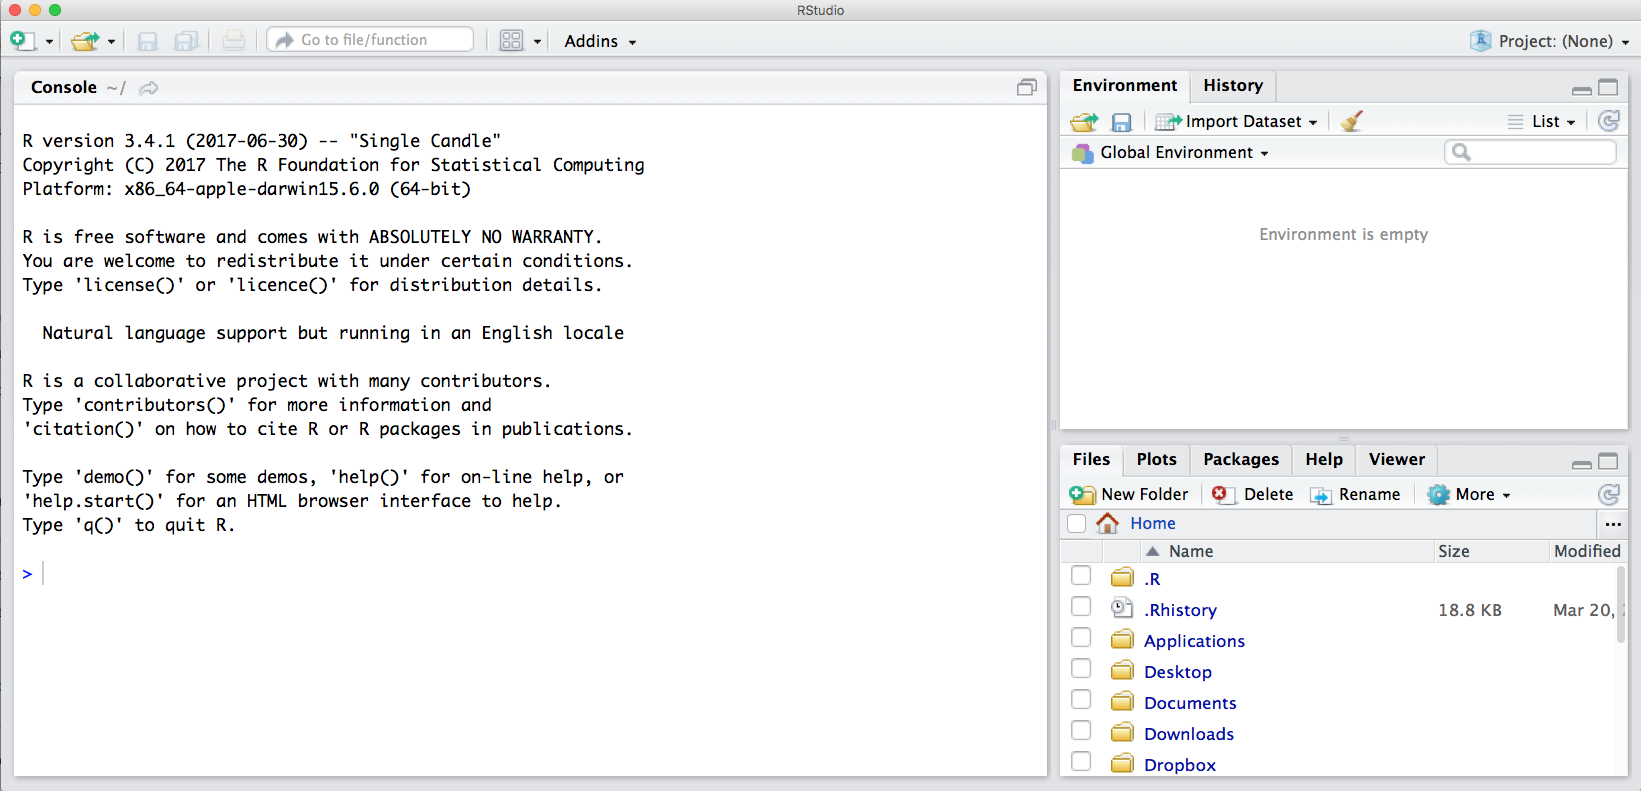
\includegraphics{img/RStudio_IDE.png}

Notice the default panes:

\begin{itemize}
\tightlist
\item
  Console (entire left)
\item
  Environment/History (tabbed in upper right)
\item
  Files/Plots/Packages/Help (tabbed in lower right)
\end{itemize}

FYI: you can change the default location of the panes, among many other things: \href{https://support.rstudio.com/hc/en-us/articles/200549016-Customizing-RStudio}{Customizing RStudio}.

An important first question: \textbf{where are we?}

If you've have opened RStudio for the first time, you'll be in your Home directory. This is noted by the \texttt{\textasciitilde{}/} at the top of the console. You can see too that the Files pane in the lower right shows what is in the Home directory where you are. You can navigate around within that Files pane and explore, but note that you won't change where you are: even as you click through you'll still be Home: \texttt{\textasciitilde{}/}.

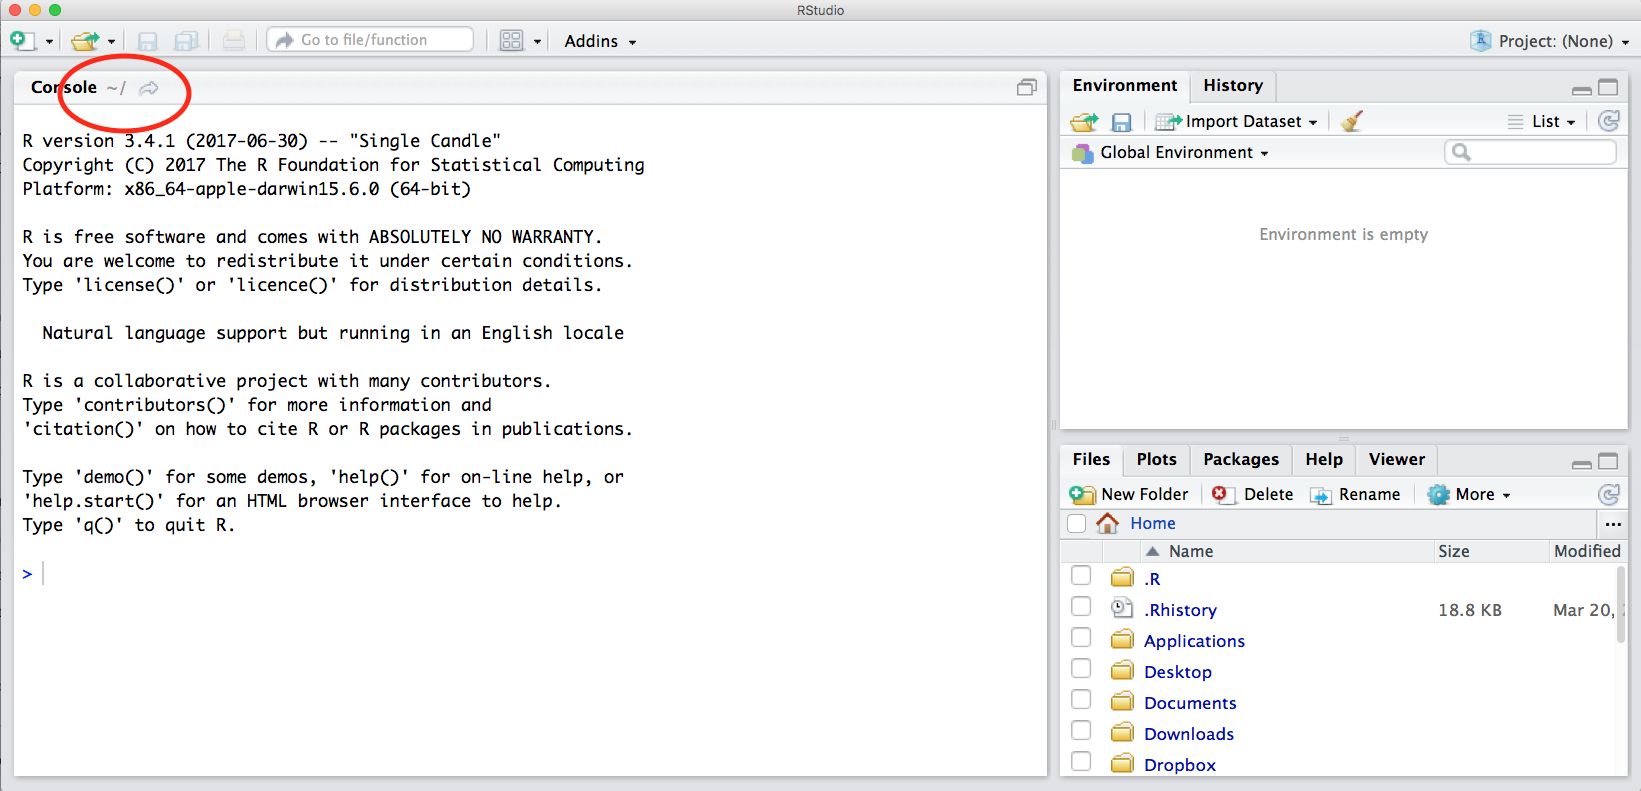
\includegraphics{img/RStudio_IDE_homedir.png}

\hypertarget{rstudio-projects}{%
\subsection{RStudio Projects}\label{rstudio-projects}}

Create a new project called `RforExcelUsers'. Why does this matter? Working directory = no file path/broken path issues. Notice that a folder now appears wherever you saved this project with the same name, and it contains a .Rproj file.

Let's do this together (with screenshots).

Important question: where are we? Now we are in this project. Everything we do will by default be saved here so we can be nice and organized.

\hypertarget{r-console}{%
\subsection{R Console}\label{r-console}}

Watch me work in the console.

I can do math, I can store data in variables, and recall those variables.

There are also functions like in Excel; I can do \texttt{?sum} and look at the help pages.

OK so working in the Console is great, but it gets messy. It's good for quick things. But looking back at what I've done and trying to build upon it would be a nightmare.

\hypertarget{deep-thought-error-messages-are-your-friends}{%
\subsection{Deep thought: Error messages are your friends}\label{deep-thought-error-messages-are-your-friends}}

Implicit contract with the computer / scripting language: Computer will do tedious computation for you. In return, you will be completely precise in your instructions. Typos matter. Case matters. Pay attention to how you type.

Remember that this is a language, not unsimilar to English! There are times you aren't understood -- it's going to happen. There are different ways this can happen. Sometimes you'll get an error. This is like someone saying `What?' or `Pardon'? Error messages can also be more useful, like when they say `I didn't understand what you said, I was expecting you to say blah'. That is a great type of error message. Error messages are your friend. Google them (copy-and-paste!) to figure out what they mean.

---\textgreater{}

And also know that there are errors that can creep in more subtly, when you are giving information that is understood, but not in the way you meant. Like if I am telling a story about suspenders that my British friend hears but silently interprets in a very different way (true story). This can leave me thinking I've gotten something across that the listener (or R) might silently interpreted very differently. And as I continue telling my story you get more and more confused\ldots{} Clear communication is critical when you code: write clean, well documented code and check your work as you go to minimize these circumstances!

\hypertarget{r-scripts}{%
\section{R Scripts}\label{r-scripts}}

Instead of working in the Console that can get messy, we can be more organized. In a script. Let's all do this together.

File \textgreater{} New File \textgreater{} R Script.

This is a blank slate for us to write our code; but there are some good practices we can start off with. Let's add a useful header to the top of it. For example, at a minimum:

\begin{Shaded}
\begin{Highlighting}[]
\CommentTok{# --------------------------------}
\CommentTok{# A descriptive title}
\CommentTok{# Summary of what this script is for }
\CommentTok{# Your name}
\CommentTok{# Contact information}
\CommentTok{# Date}
\CommentTok{# --------------------------------}

\CommentTok{# Other things you might include: required packages or datasets, relevant links (e.g. to raw data source, GitHub repo, etc.), citations and sources.}
\end{Highlighting}
\end{Shaded}

Since we're working in or Project, this script is now nicely saved in our Project

Let's attach a package. Since you've already installed tidyverse

Cool looking plot with diamonds.

You can run code line by line or sourcing the script

\hypertarget{dont-save-the-workspace}{%
\section{Don't save the workspace}\label{dont-save-the-workspace}}

\hypertarget{deep-thought-keep-the-raw-data-raw.}{%
\section{Deep thought: keep the raw data raw.}\label{deep-thought-keep-the-raw-data-raw.}}

Discussing using Excel for variables.

\hypertarget{interludes-deep-thoughtsopenscapes}{%
\section{Interludes (deep thoughts/openscapes)}\label{interludes-deep-thoughtsopenscapes}}

Comments! Organization (spacing, subsections, vertical structure, indentation, etc.)! Well-named variables! Also, well-named operations so analyses (select(data, columnname)) instead of data{[}1:6,5{]} and excel equivalent. (Ex with strings)
Not so brittle/sensitive to minor changes.

\hypertarget{our-turn-your-turn-1}{%
\section{Our Turn Your Turn 1}\label{our-turn-your-turn-1}}

\hypertarget{our-turn-your-turn-2}{%
\section{Our Turn Your Turn 2}\label{our-turn-your-turn-2}}

\hypertarget{efficiency-tips}{%
\section{Efficiency Tips}\label{efficiency-tips}}

\hypertarget{readxl}{%
\chapter{\texorpdfstring{\texttt{readxl}}{readxl}}\label{readxl}}

Note for Allison: the \texttt{\{\#readxl\}} above lets us reference it from another chapter\ldots{}not sure how much we'll use it but it's possible (and doesn't hurt to have). Cool, thanks Julie!

\hypertarget{summary-a-few-sentences-1}{%
\section{Summary (a few sentences)}\label{summary-a-few-sentences-1}}

The \textbf{readxl} package makes it easy to import tabular data from Excel spreadsheets (.xls or .xlsx files) and includes several options for cleaning data during import. \textbf{readxl} has no external dependencies and functions on any operating system, making it an OS- and user-friendly package that simplifies getting your data from Excel into R.

\hypertarget{objectives-more-detailed-bulletpoints-1}{%
\section{Objectives (more detailed, bulletpoints?)}\label{objectives-more-detailed-bulletpoints-1}}

\begin{itemize}
\tightlist
\item
  Use readr::read\_csv() to read in a comma separated value (CSV) file
\item
  Use readxl::read\_excel() to read in an Excel worksheet
\item
  Use readxl::read\_excel() to read in parts of a worksheet (by cell range)
\item
  Specify column names when importing Excel data
\item
  Replace a specific string/value in a spreadsheet with with `NA'
\item
  Skip \emph{n} rows when importing an Excel worksheet
\item
  Read in multiple Excel worksheets
\item
  Something about readxl workflows (e.g. \%\textgreater{}\% write\_csv() to keep a copy of the raw data in a project)??
\end{itemize}

\hypertarget{resources-1}{%
\section{Resources}\label{resources-1}}

\begin{itemize}
\tightlist
\item
  \url{https://readxl.tidyverse.org/}
\end{itemize}

\hypertarget{lessons-teaching-for-each-objective..-objectives-examples}{%
\section{Lessons teaching for each objective\ldots{}.. (objectives, examples)}\label{lessons-teaching-for-each-objective..-objectives-examples}}

\hypertarget{prep-get-data-files-into-your-working-directory}{%
\subsection{Prep: get data files into your working directory}\label{prep-get-data-files-into-your-working-directory}}

In Session 1, we introduced how and why R Projects are great for reproducibility, because our self-contained working directory will be the \textbf{first} place R looks for files.

You downloaded four files for this workshop:

\begin{itemize}
\tightlist
\item
  fish\_counts\_curated.csv
\item
  invert\_counts\_curated.xlsx
\item
  kelp\_counts\_curated.xlsx
\item
  \ldots{}the OTHER ONE?
\end{itemize}

Copy and paste those files into the `RforExcelUsers' folder on your computer. Notice that now these files show up right in your working directory when you go back to that Project in RStudio! That means they're going to be in the first place R will look when you ask it to find a file.

\hypertarget{create-a-new-.r-script-and-attach-the-tidyverse}{%
\subsection{Create a new .R script and attach the tidyverse}\label{create-a-new-.r-script-and-attach-the-tidyverse}}

In your RforExcelUsers project in RStudio, open a new .R script and add a useful header to the top of it. For example, at a minimum:

\begin{Shaded}
\begin{Highlighting}[]
\CommentTok{# --------------------------------}
\CommentTok{# A descriptive title}
\CommentTok{# Summary of what this script is for }
\CommentTok{# Your name}
\CommentTok{# Contact information}
\CommentTok{# --------------------------------}

\CommentTok{# Other things you might include: required packages or datasets, relevant links (e.g. to raw data source, GitHub repo, etc.), citations and sources.}
\end{Highlighting}
\end{Shaded}

We'll read in a CSV file with \texttt{readr::read\_csv()}, so we need to have the \texttt{readr} package attached. Since it's part of the \texttt{tidyverse}, we'll go ahead and attach the \texttt{tidyverse} package below our script header using \texttt{library(package\_name)}.

\begin{Shaded}
\begin{Highlighting}[]
\CommentTok{# Attach the tidyverse}
\KeywordTok{library}\NormalTok{(tidyverse)}
\end{Highlighting}
\end{Shaded}

Now, all of the packages and functions within the \texttt{tidyverse}, including \texttt{readr::read\_csv()} are available for us to use.

\hypertarget{use-readrread_csv-to-read-in-data-from-a-csv-file}{%
\subsection{\texorpdfstring{Use \textbf{readr::read\_csv()} to read in data from a CSV file}{Use readr::read\_csv() to read in data from a CSV file}}\label{use-readrread_csv-to-read-in-data-from-a-csv-file}}

There are many types of files containing data that you might want to work with in R. A common one is a comma separated value (CSV) file, which contains values with each column entry separated by a comma delimiter. CSVs can be opened, viewed, and worked with in Excel just like an .xls or .xlsx file - but let's learn how to get data directly from a CSV into R where we can work with it more reproducibly.

The CSV we'll read in here is called ``fish\_counts\_curated.csv'', and contains observations for ``the abundance and size of fish species as part of SBCLTER's kelp forest monitoring program to track long-term patterns in species abundance and diversity'' from the \href{http://sbc.lternet.edu/}{Santa Barbara Channel Long Term Ecological Research} program.

\textbf{Source:} Reed D. 2018. SBC LTER: Reef: Kelp Forest Community Dynamics: Fish abundance. Environmental Data Initiative. \url{https://doi.org/10.6073/pasta/dbd1d5f0b225d903371ce89b09ee7379}. Dataset accessed 9/26/2019.

Read in the ``fish\_counts\_curated.csv''

\hypertarget{fun-facts-quirky-things---making-a-note-of-these-wherever-possible-for-interest-little-did-you-know-sections}{%
\section{Fun facts (quirky things) - making a note of these wherever possible for interest (little ``Did you know?'' sections)}\label{fun-facts-quirky-things---making-a-note-of-these-wherever-possible-for-interest-little-did-you-know-sections}}

\hypertarget{interludes-deep-thoughtsopenscapes-1}{%
\section{Interludes (deep thoughts/openscapes)}\label{interludes-deep-thoughtsopenscapes-1}}

\hypertarget{our-turn-your-turn-1-1}{%
\section{Our Turn Your Turn 1}\label{our-turn-your-turn-1-1}}

\hypertarget{our-turn-your-turn-2-1}{%
\section{Our Turn Your Turn 2}\label{our-turn-your-turn-2-1}}

\hypertarget{efficiency-tips-1}{%
\section{Efficiency Tips}\label{efficiency-tips-1}}

\hypertarget{rmarkdown}{%
\chapter{RMarkdown}\label{rmarkdown}}

\hypertarget{summary-a-few-sentences-2}{%
\section{Summary (a few sentences)}\label{summary-a-few-sentences-2}}

\hypertarget{objectives-more-detailed-bulletpoints-2}{%
\section{Objectives (more detailed, bulletpoints?)}\label{objectives-more-detailed-bulletpoints-2}}

\hypertarget{resources-2}{%
\section{Resources}\label{resources-2}}

\hypertarget{lessons-teaching-for-each-objective..-objectives-examples-1}{%
\section{Lessons teaching for each objective\ldots{}.. (objectives, examples)}\label{lessons-teaching-for-each-objective..-objectives-examples-1}}

\hypertarget{fun-facts-quirky-things---making-a-note-of-these-wherever-possible-for-interest-little-did-you-know-sections-1}{%
\section{Fun facts (quirky things) - making a note of these wherever possible for interest (little ``Did you know?'' sections)}\label{fun-facts-quirky-things---making-a-note-of-these-wherever-possible-for-interest-little-did-you-know-sections-1}}

\hypertarget{interludes-deep-thoughtsopenscapes-2}{%
\section{Interludes (deep thoughts/openscapes)}\label{interludes-deep-thoughtsopenscapes-2}}

\hypertarget{our-turn-your-turn-1-2}{%
\section{Our Turn Your Turn 1}\label{our-turn-your-turn-1-2}}

\hypertarget{our-turn-your-turn-2-2}{%
\section{Our Turn Your Turn 2}\label{our-turn-your-turn-2-2}}

\hypertarget{efficiency-tips-2}{%
\section{Efficiency Tips}\label{efficiency-tips-2}}

\hypertarget{pivot}{%
\chapter{Dplyr and Pivot Tables}\label{pivot}}

\hypertarget{summary-a-few-sentences-3}{%
\section{Summary (a few sentences)}\label{summary-a-few-sentences-3}}

\hypertarget{objectives-more-detailed-bulletpoints-3}{%
\section{Objectives (more detailed, bulletpoints?)}\label{objectives-more-detailed-bulletpoints-3}}

\hypertarget{resources-3}{%
\section{Resources}\label{resources-3}}

\hypertarget{lessons-teaching-for-each-objective..-objectives-examples-2}{%
\section{Lessons teaching for each objective\ldots{}.. (objectives, examples)}\label{lessons-teaching-for-each-objective..-objectives-examples-2}}

\hypertarget{fun-facts-quirky-things---making-a-note-of-these-wherever-possible-for-interest-little-did-you-know-sections-2}{%
\section{Fun facts (quirky things) - making a note of these wherever possible for interest (little ``Did you know?'' sections)}\label{fun-facts-quirky-things---making-a-note-of-these-wherever-possible-for-interest-little-did-you-know-sections-2}}

\hypertarget{interludes-deep-thoughtsopenscapes-3}{%
\section{Interludes (deep thoughts/openscapes)}\label{interludes-deep-thoughtsopenscapes-3}}

\hypertarget{our-turn-your-turn-1-3}{%
\section{Our Turn Your Turn 1}\label{our-turn-your-turn-1-3}}

\hypertarget{our-turn-your-turn-2-3}{%
\section{Our Turn Your Turn 2}\label{our-turn-your-turn-2-3}}

\hypertarget{efficiency-tips-3}{%
\section{Efficiency Tips}\label{efficiency-tips-3}}

\hypertarget{vlookup}{%
\chapter{Dplyr and vlookups}\label{vlookup}}

\hypertarget{summary-a-few-sentences-4}{%
\section{Summary (a few sentences)}\label{summary-a-few-sentences-4}}

\hypertarget{objectives-more-detailed-bulletpoints-4}{%
\section{Objectives (more detailed, bulletpoints?)}\label{objectives-more-detailed-bulletpoints-4}}

\hypertarget{resources-4}{%
\section{Resources}\label{resources-4}}

\hypertarget{lessons-teaching-for-each-objective..-objectives-examples-3}{%
\section{Lessons teaching for each objective\ldots{}.. (objectives, examples)}\label{lessons-teaching-for-each-objective..-objectives-examples-3}}

\hypertarget{fun-facts-quirky-things---making-a-note-of-these-wherever-possible-for-interest-little-did-you-know-sections-3}{%
\section{Fun facts (quirky things) - making a note of these wherever possible for interest (little ``Did you know?'' sections)}\label{fun-facts-quirky-things---making-a-note-of-these-wherever-possible-for-interest-little-did-you-know-sections-3}}

\hypertarget{interludes-deep-thoughtsopenscapes-4}{%
\section{Interludes (deep thoughts/openscapes)}\label{interludes-deep-thoughtsopenscapes-4}}

\hypertarget{our-turn-your-turn-1-4}{%
\section{Our Turn Your Turn 1}\label{our-turn-your-turn-1-4}}

\hypertarget{our-turn-your-turn-2-4}{%
\section{Our Turn Your Turn 2}\label{our-turn-your-turn-2-4}}

\hypertarget{efficiency-tips-4}{%
\section{Efficiency Tips}\label{efficiency-tips-4}}

\hypertarget{tidying}{%
\chapter{Tidying}\label{tidying}}

\hypertarget{better-practices-needs-a-better-name}{%
\section{Better practices {[}needs a better name{]}}\label{better-practices-needs-a-better-name}}

How to be a nimble useR
Modern useRs are nimble internet useRs
something clever about cleaning
I am the worst at naming things

\hypertarget{summary-a-few-sentences-5}{%
\section{Summary (a few sentences)}\label{summary-a-few-sentences-5}}

R ecosystem evolves and improves due to contributed work by the community, and this is a good thing. Being a nimble useR means being able to navigate/keep tabs on this ecosystem and find what you need. It also means working reproducibly, so you can re-run and update things more easily. Here we will teach you how to expect things and help yourself. Pay attention to urls.

\hypertarget{objectives-more-detailed-bulletpoints-5}{%
\section{Objectives (more detailed, bulletpoints?)}\label{objectives-more-detailed-bulletpoints-5}}

\begin{itemize}
\tightlist
\item
  expect there is a better way, how and where to look (20 mins)

  \begin{itemize}
  \tightlist
  \item
    CRAN
  \item
    Twitter \#rstats
  \item
    rOpenSci
  \item
    RStudio
  \item
    Example: how to Google.
  \end{itemize}
\item
  hands-on with janitor (30+ mins)

  \begin{itemize}
  \tightlist
  \item
    discovery and quality assurance
  \item
    installing from GitHub
  \item
    big payoff for little effort
  \end{itemize}
\item
  hands-on with another excel-useful example: skimr?\\
\item
  reproducibility (20 mins)

  \begin{itemize}
  \tightlist
  \item
    it's important, scripted
  \end{itemize}
\end{itemize}

\hypertarget{resources-5}{%
\section{Resources}\label{resources-5}}

\begin{itemize}
\tightlist
\item
  Wilson et al.~2014 ``Good enough practices''
\end{itemize}

\hypertarget{lessons-teaching-for-each-objective..-objectives-examples-4}{%
\section{Lessons teaching for each objective\ldots{}.. (objectives, examples)}\label{lessons-teaching-for-each-objective..-objectives-examples-4}}

\hypertarget{expect-theres-a-better-way-chat}{%
\subsection{Expect there's a better way chat}\label{expect-theres-a-better-way-chat}}

\begin{itemize}
\tightlist
\item
  give time for them to google?
\end{itemize}

\hypertarget{janitor}{%
\subsection{Janitor}\label{janitor}}

janitor \& other things that will make your life easier with limited effort
Janitor: up till now the column names have been fine. Until now.

\hypertarget{our-turn-your-turn}{%
\subsubsection{Our turn your turn}\label{our-turn-your-turn}}

Walk through and example and leave our code up, and have you do it but clean another dataset. Work with a neighbor.

\hypertarget{example-how-to-google}{%
\subsection{Example: How to Google}\label{example-how-to-google}}

Pay attention to URLs, build github/rmarkdown savviness (ex: raw.githubusercontent.com)

\begin{itemize}
\tightlist
\item
  I read this blog: \url{https://blog.revolutionanalytics.com/2018/08/how-to-use-r-with-excel.html}
\item
  I've never heard of click on \texttt{openxlsx}, what is it
\item
  Takes me here \url{https://www.rdocumentation.org/packages/openxlsx/versions/4.1.0.1}, but I want more info. How recently was it worked on? Does it interface with tidyverse? Click on ``news''
\item
  Takes me here. \url{https://raw.githubusercontent.com/awalker89/openxlsx/master/NEWS} . Not useful. But from this URL, - I see the username so I can edit this url to be
  \url{https://github.com/awalker89/openxlsx/}
\item
  1st thing: most recent commit was a year ago. Can poke around more, are there issues open, are they taken care of? Etc. I will probably not pursue using this right now. But good to have learned about it.
\end{itemize}

\hypertarget{fun-facts-quirky-things---making-a-note-of-these-wherever-possible-for-interest-little-did-you-know-sections-4}{%
\section{Fun facts (quirky things) - making a note of these wherever possible for interest (little ``Did you know?'' sections)}\label{fun-facts-quirky-things---making-a-note-of-these-wherever-possible-for-interest-little-did-you-know-sections-4}}

\hypertarget{interludes-deep-thoughtsopenscapes-5}{%
\section{Interludes (deep thoughts/openscapes)}\label{interludes-deep-thoughtsopenscapes-5}}

\hypertarget{our-turn-your-turn-2-5}{%
\section{Our Turn Your Turn 2}\label{our-turn-your-turn-2-5}}

\hypertarget{efficiency-tips-5}{%
\section{Efficiency Tips}\label{efficiency-tips-5}}

\begin{itemize}
\tightlist
\item
  browser efficiency tips

  \begin{itemize}
  \tightlist
  \item
    Rmd/github anchors for urls
  \item
    press command to open a new tab
  \end{itemize}
\end{itemize}

Reproducibility is important (this might be new to some people)
Example: run everything start to finish and then closing it all and trying to do again
In excel
Vs R
If your computer shuts off are you nervous to close it?
Recreate it
``What they didn't forget to teach you about R'' WTDF. uncool

\hypertarget{format}{%
\chapter{Formatting and Sharing}\label{format}}

\hypertarget{summary-a-few-sentences-6}{%
\section{Summary (a few sentences)}\label{summary-a-few-sentences-6}}

\hypertarget{objectives-more-detailed-bulletpoints-6}{%
\section{Objectives (more detailed, bulletpoints?)}\label{objectives-more-detailed-bulletpoints-6}}

\hypertarget{resources-6}{%
\section{Resources}\label{resources-6}}

\hypertarget{lessons-teaching-for-each-objective..-objectives-examples-5}{%
\section{Lessons teaching for each objective\ldots{}.. (objectives, examples)}\label{lessons-teaching-for-each-objective..-objectives-examples-5}}

\begin{enumerate}
\def\labelenumi{\arabic{enumi}.}
\tightlist
\item
  Create a GitHub account: \url{https://github.com} \emph{Note! Shorter names that kind of identify you are better, and use your work email!}
\end{enumerate}

\hypertarget{fun-facts-quirky-things---making-a-note-of-these-wherever-possible-for-interest-little-did-you-know-sections-5}{%
\section{Fun facts (quirky things) - making a note of these wherever possible for interest (little ``Did you know?'' sections)}\label{fun-facts-quirky-things---making-a-note-of-these-wherever-possible-for-interest-little-did-you-know-sections-5}}

\hypertarget{interludes-deep-thoughtsopenscapes-6}{%
\section{Interludes (deep thoughts/openscapes)}\label{interludes-deep-thoughtsopenscapes-6}}

\hypertarget{our-turn-your-turn-1-5}{%
\section{Our Turn Your Turn 1}\label{our-turn-your-turn-1-5}}

\hypertarget{our-turn-your-turn-2-6}{%
\section{Our Turn Your Turn 2}\label{our-turn-your-turn-2-6}}

\hypertarget{efficiency-tips-6}{%
\section{Efficiency Tips}\label{efficiency-tips-6}}

\hypertarget{synthesis}{%
\chapter{Synthesis}\label{synthesis}}

\hypertarget{summary-a-few-sentences-7}{%
\section{Summary (a few sentences)}\label{summary-a-few-sentences-7}}

\hypertarget{objectives-more-detailed-bulletpoints-7}{%
\section{Objectives (more detailed, bulletpoints?)}\label{objectives-more-detailed-bulletpoints-7}}

\hypertarget{resources-7}{%
\section{Resources}\label{resources-7}}

\hypertarget{lessons-teaching-for-each-objective..-objectives-examples-6}{%
\section{Lessons teaching for each objective\ldots{}.. (objectives, examples)}\label{lessons-teaching-for-each-objective..-objectives-examples-6}}

\hypertarget{fun-facts-quirky-things---making-a-note-of-these-wherever-possible-for-interest-little-did-you-know-sections-6}{%
\section{Fun facts (quirky things) - making a note of these wherever possible for interest (little ``Did you know?'' sections)}\label{fun-facts-quirky-things---making-a-note-of-these-wherever-possible-for-interest-little-did-you-know-sections-6}}

\hypertarget{interludes-deep-thoughtsopenscapes-7}{%
\section{Interludes (deep thoughts/openscapes)}\label{interludes-deep-thoughtsopenscapes-7}}

\hypertarget{our-turn-your-turn-1-6}{%
\section{Our Turn Your Turn 1}\label{our-turn-your-turn-1-6}}

\hypertarget{our-turn-your-turn-2-7}{%
\section{Our Turn Your Turn 2}\label{our-turn-your-turn-2-7}}

\hypertarget{efficiency-tips-7}{%
\section{Efficiency Tips}\label{efficiency-tips-7}}

\bibliography{book.bib,packages.bib}


\end{document}
